%!TEX root = ../dokumentation.tex

\chapter{Projektziel}

Betrachtet man weltweit die aktuell größten IT-Firmen und Start-ups, so fällt schnell auf, dass diese überwiegend auf dem gleichen Konzept aufgebaut sind.
Egal ob Amazon, Spotify oder Netflix, besteht das zentrale Angebot dieser Firmen aus einer Plattform, die als Anlaufstelle für ein vorherig schwer zu navigierendes Medium genutzt wird.
Bei Spotify findet man an einer Stelle alle Lieder und zusätzlich erleichtert die Plattform das Auffinden von neuen Genres und Musikern.
Netflix und Amazon haben ähnliche Konzepte was Filme und (physische) Einkaufswaren angeht.
Ziel dieses Projektes soll es sein eine solche Plattform für RSS Feeds und den darin übermittelten Artikeln zu erstellen.
Das Projekt \enquote{Skiosa} soll eine Plattform anbieten, die zur zentralen Anlaufstelle für RSS Feeds agieren kann und so ihren Nutzern das Entdecken von neuen Artikeln aus bekannten, sowie unbekannten Feeds erleichtert.

\section{Projektanforderungen}

Im Folgenden soll nun beschrieben werden, wie zu Anfang des Projektes die Requirements aufgefasst und beschreiben wurden.
Aus technischen Gründen hat sich im Verlauf des Prozesses herausgestellt, dass einige dieser Requirements nicht so implementierbar sind und wurden daher leicht abgeändert.
Mehr Informationen hierzu sind im Abschnitt \ref{tech_changes} nachzulesen.

\subsection{Unverzichtbare Ziele}
Zu Begin müssen zentrale Interaktionsmechanismen für Artikel und Feeds gegeben sein.
Seiten für das Einsehen von Artikeln und Feeds bilden daher den Kern der Applikation.
% NOTE: INHALT wurde rausgestrichen und warum muss in section \ref{tech_changes} erklärt werden
Auf den Einsichtsseiten für Artikel und Feeds muss es möglich sein Basisinformationen, wie etwa Titel, Inhalt oder Beschreibung, nachlesen zu können.
Bei Artikeln muss die Einsichtsseite zusätzlich auf den eigentlichen Artikel verweisen, während bei Feeds auf die in ihnen enthaltenen Artikel verlinkt wird.

Den größten Mehrwert der Plattform sollen vorgeschlagene Artikel bilden.
Es soll Nutzern möglich sein innerhalb der Plattform neue Artikel zu entdecken.
Funktional bedeutet dies, dass die wichtigste Anforderung an die Plattform eine Seite ist, auf welcher (sich ständig erneuernde) Vorschläge für Artikel abgebildet sind.

Damit Skiosa zu einer zentralen Anlaufstelle für RSS-Feeds werden kann, müssen Nutzer einen Grund haben um wiederholt auf die Plattform zugreifen zu wollen.
Subscription\footnote{dt. Abonnement}- und Bookmark\footnote{dt. Vermerk}-Funktionalitäten für eingeloggte Nutzer können genau diese Lücke füllen.
Hieraus leiten sich drei weitere funktionale Requirements ab:
Erstens muss die Plattform ein User-Management besitzen, in welcher sich Nutzer einloggen und registrieren können.
Zweitens soll es angemeldeten Nutzern der Plattform möglich sein, bestimmte Feeds zu abonnieren und diese, sowie deren neusten Artikeln, im Nachhinein aufzurufen zu können.
Drittens sollen angemeldeten Nutzer Artikel \enquote{bookmarken} (dt. vermerken) können und diese zu einem späteren Zeitpunkt in der Plattform wieder finden.

Auf nicht-funktionaler Ebene ist es für die Plattform wichtig, dass diese ästhetisch gut aussieht.
Konkrete nicht-funktionale Requirements, die sich hieraus ableiten sind, dass die Oberflächen der Plattform einer festen Design-Sprache folgen und User Experience Design seitenübergreifen einheitlich gestaltet ist.

\subsection{Erreichbare Ziele}
Zusätzlich für das Projekt hilfreiche Funktionalitäten, die zu Anfang als erreichbar angesehen wurden wenden, sich um das Optimieren der vorgeschlagenen Artikeln.
Es wäre für Nutzer, die es aus bspw. Spotify oder YouTube gewohnt sind ihre Präferenzen als \enquote{Likes} anzugeben, hilfreich, wenn sie dies ebenfalls in Skiosa machen könnten.
Als optionales Requirement folgt hieraus, dass Nutzer bei Artikeln durch einen \enquote{Like}-Knopf angeben können, welche Artikel Ihnen besonders gefallen und dann ihnen mehr Artikel vorgeschlagen werden, die zu diesen ähnliche sind.

Zusätzlich ist es bei Artikeln von Zeitschriften und Blogs üblich diese einzukategorisieren.
In Skiosa wäre es hilfreich, wenn ein Benutzer diese Kategorien angeben könnten und die Vorschläge für diese Nutzer sich dann an den angegebenen Kategorien orientiert.

\subsection{Mögliche weiteren Ziele}
Eine weitere mögliche Erweiterung der Plattform, die aber im Zeitrahmen des Semesters nicht realistisch erscheint, ist das Erstellen einer Content-Management-Seite.
In dieser Content-Management-Seite könnten Besitzer von RSS Feeds ihre eigenen Feeds hinzufügen und verwalten.
Hier wäre es möglich Polling-Intervalle, Aussehen, Beschreibungen oder Titel von Feeds abzuändern.
Zusätzlich wäre es hierbei notwendig Appeal Prozesse für falsch zugewiesene Besitzer anzubieten.

Zusätzlich wäre es möglich das User-Management um Benachrichtigungseinstellungen zu erweitern. 
Hierbei könnten Benutzer der Plattform granular einstellen, ob sie Nachrichten für neue Artikel, Feeds oder Vorschläge erhalten wollen.

\section{Use Cases}
Zur Definition der Projektanforderungen wurden zusätzlich mehrere Usecase-Diagramme erstellt.

Zunächst soll der Benutzer auf einer Übersichtsseite ankommen.
Der Usecase dieser Übersichtsseite ist in der Abbildung~\ref{fig:usecaseOverview} dargestellt.
\begin{figure}
    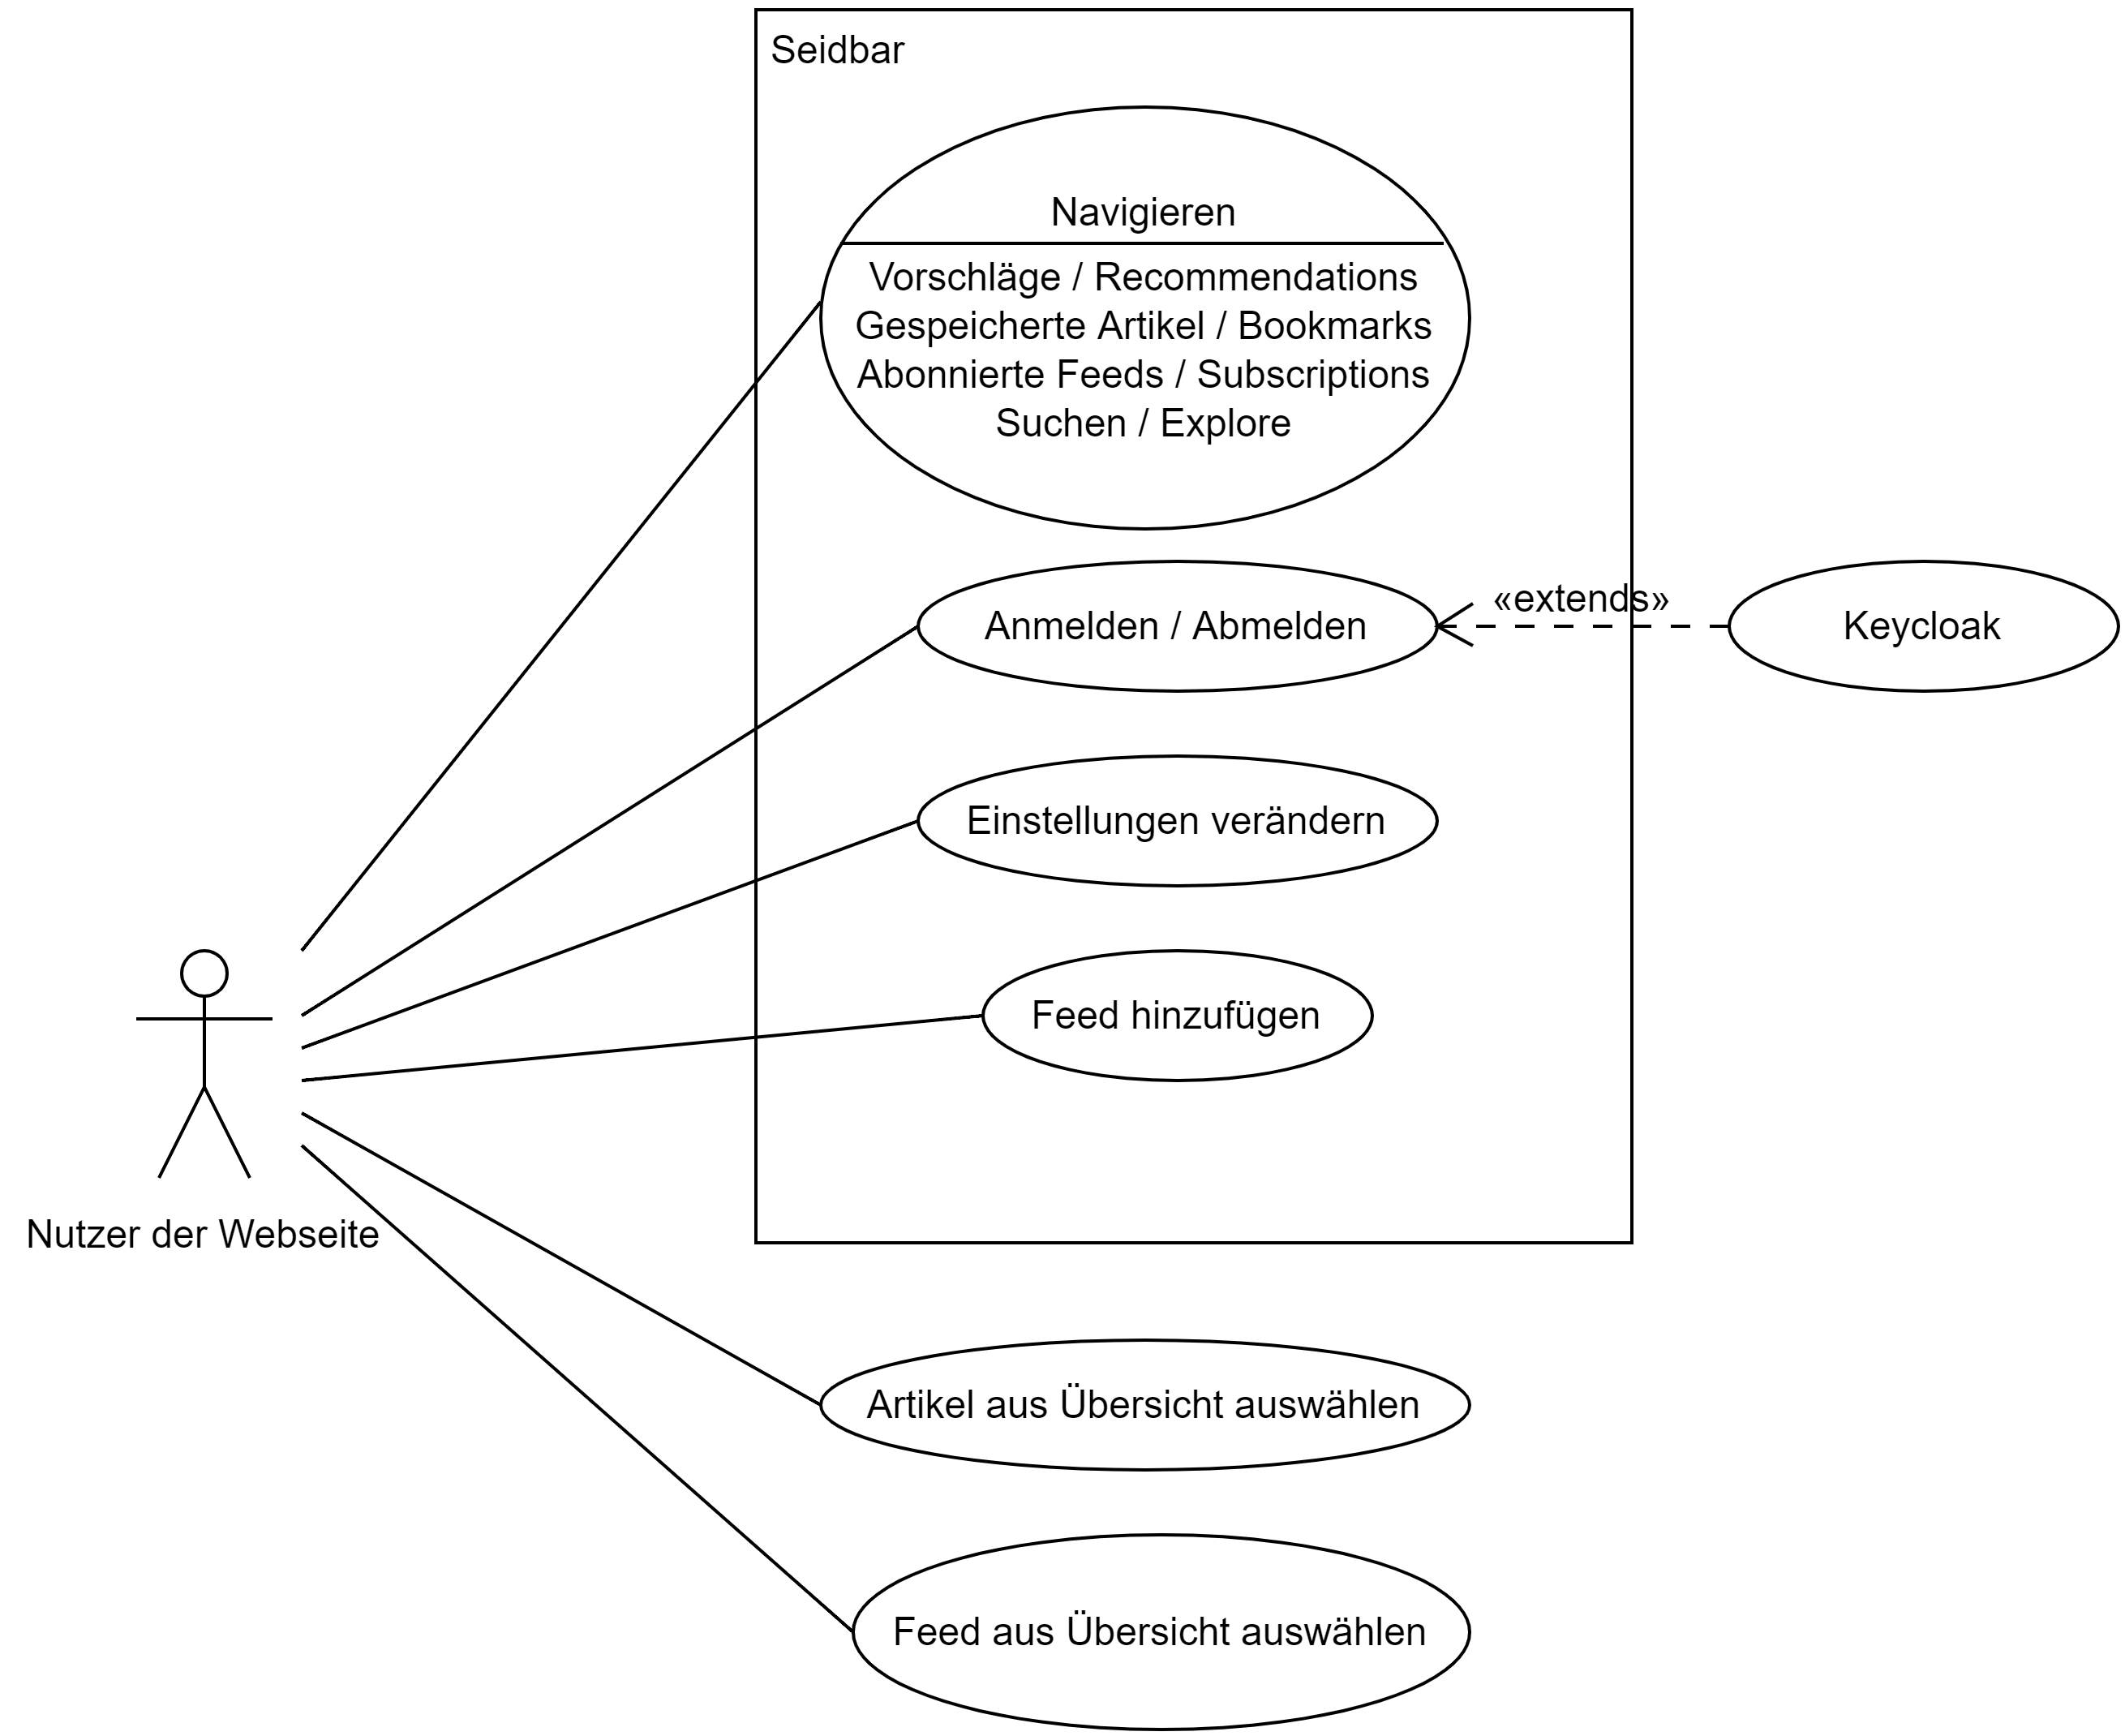
\includegraphics[width=\linewidth]{umlUsecaseOverview.png}
    \caption{Usecase Diagramm der Übersichtsseite}
    \label{fig:usecaseOverview}
\end{figure}
Auf dieser Übersichtsseite werden dem Nutzer verschiedene Feeds und Artikel angezeigt. Mit einem Klick auf einen Feed oder einen Artikel wird
der Nutzer auf eine weitere Seite weitergeleitet mit mehr Möglichkeiten. Außerdem hat der Nutzer auf der Seite über eine Sidebar die Möglichkeit
auf der Seite zu navigieren. Zusätzlich ist es in der Sidebar möglich  sich an- und abmelden, seine Usereinstellungen zu ändern, als auch neue Feeds
hinzuzufügen. 

Der Usecase der Einstellungsseite wurde in Abbildung~\ref{fig:usecaseSettings} visualisiert.
Auf dieser Seite ist ebenfalls die Sidebar sichtbar, somit sind die Interaktionen in der Sidebar dieselben, wie
bei der Übersichtsseite. Als weitere Funktionalität kann auf dieser Seite der eigene Account bearbeitet werden.
Dies soll über den externen Service Keycloak geschehen. Darüber hinaus
kann man Einstellungen zu Benachrichtigungen treffen. Das Design der
Webseite kann hier auch angepasst werden.
\begin{figure}
    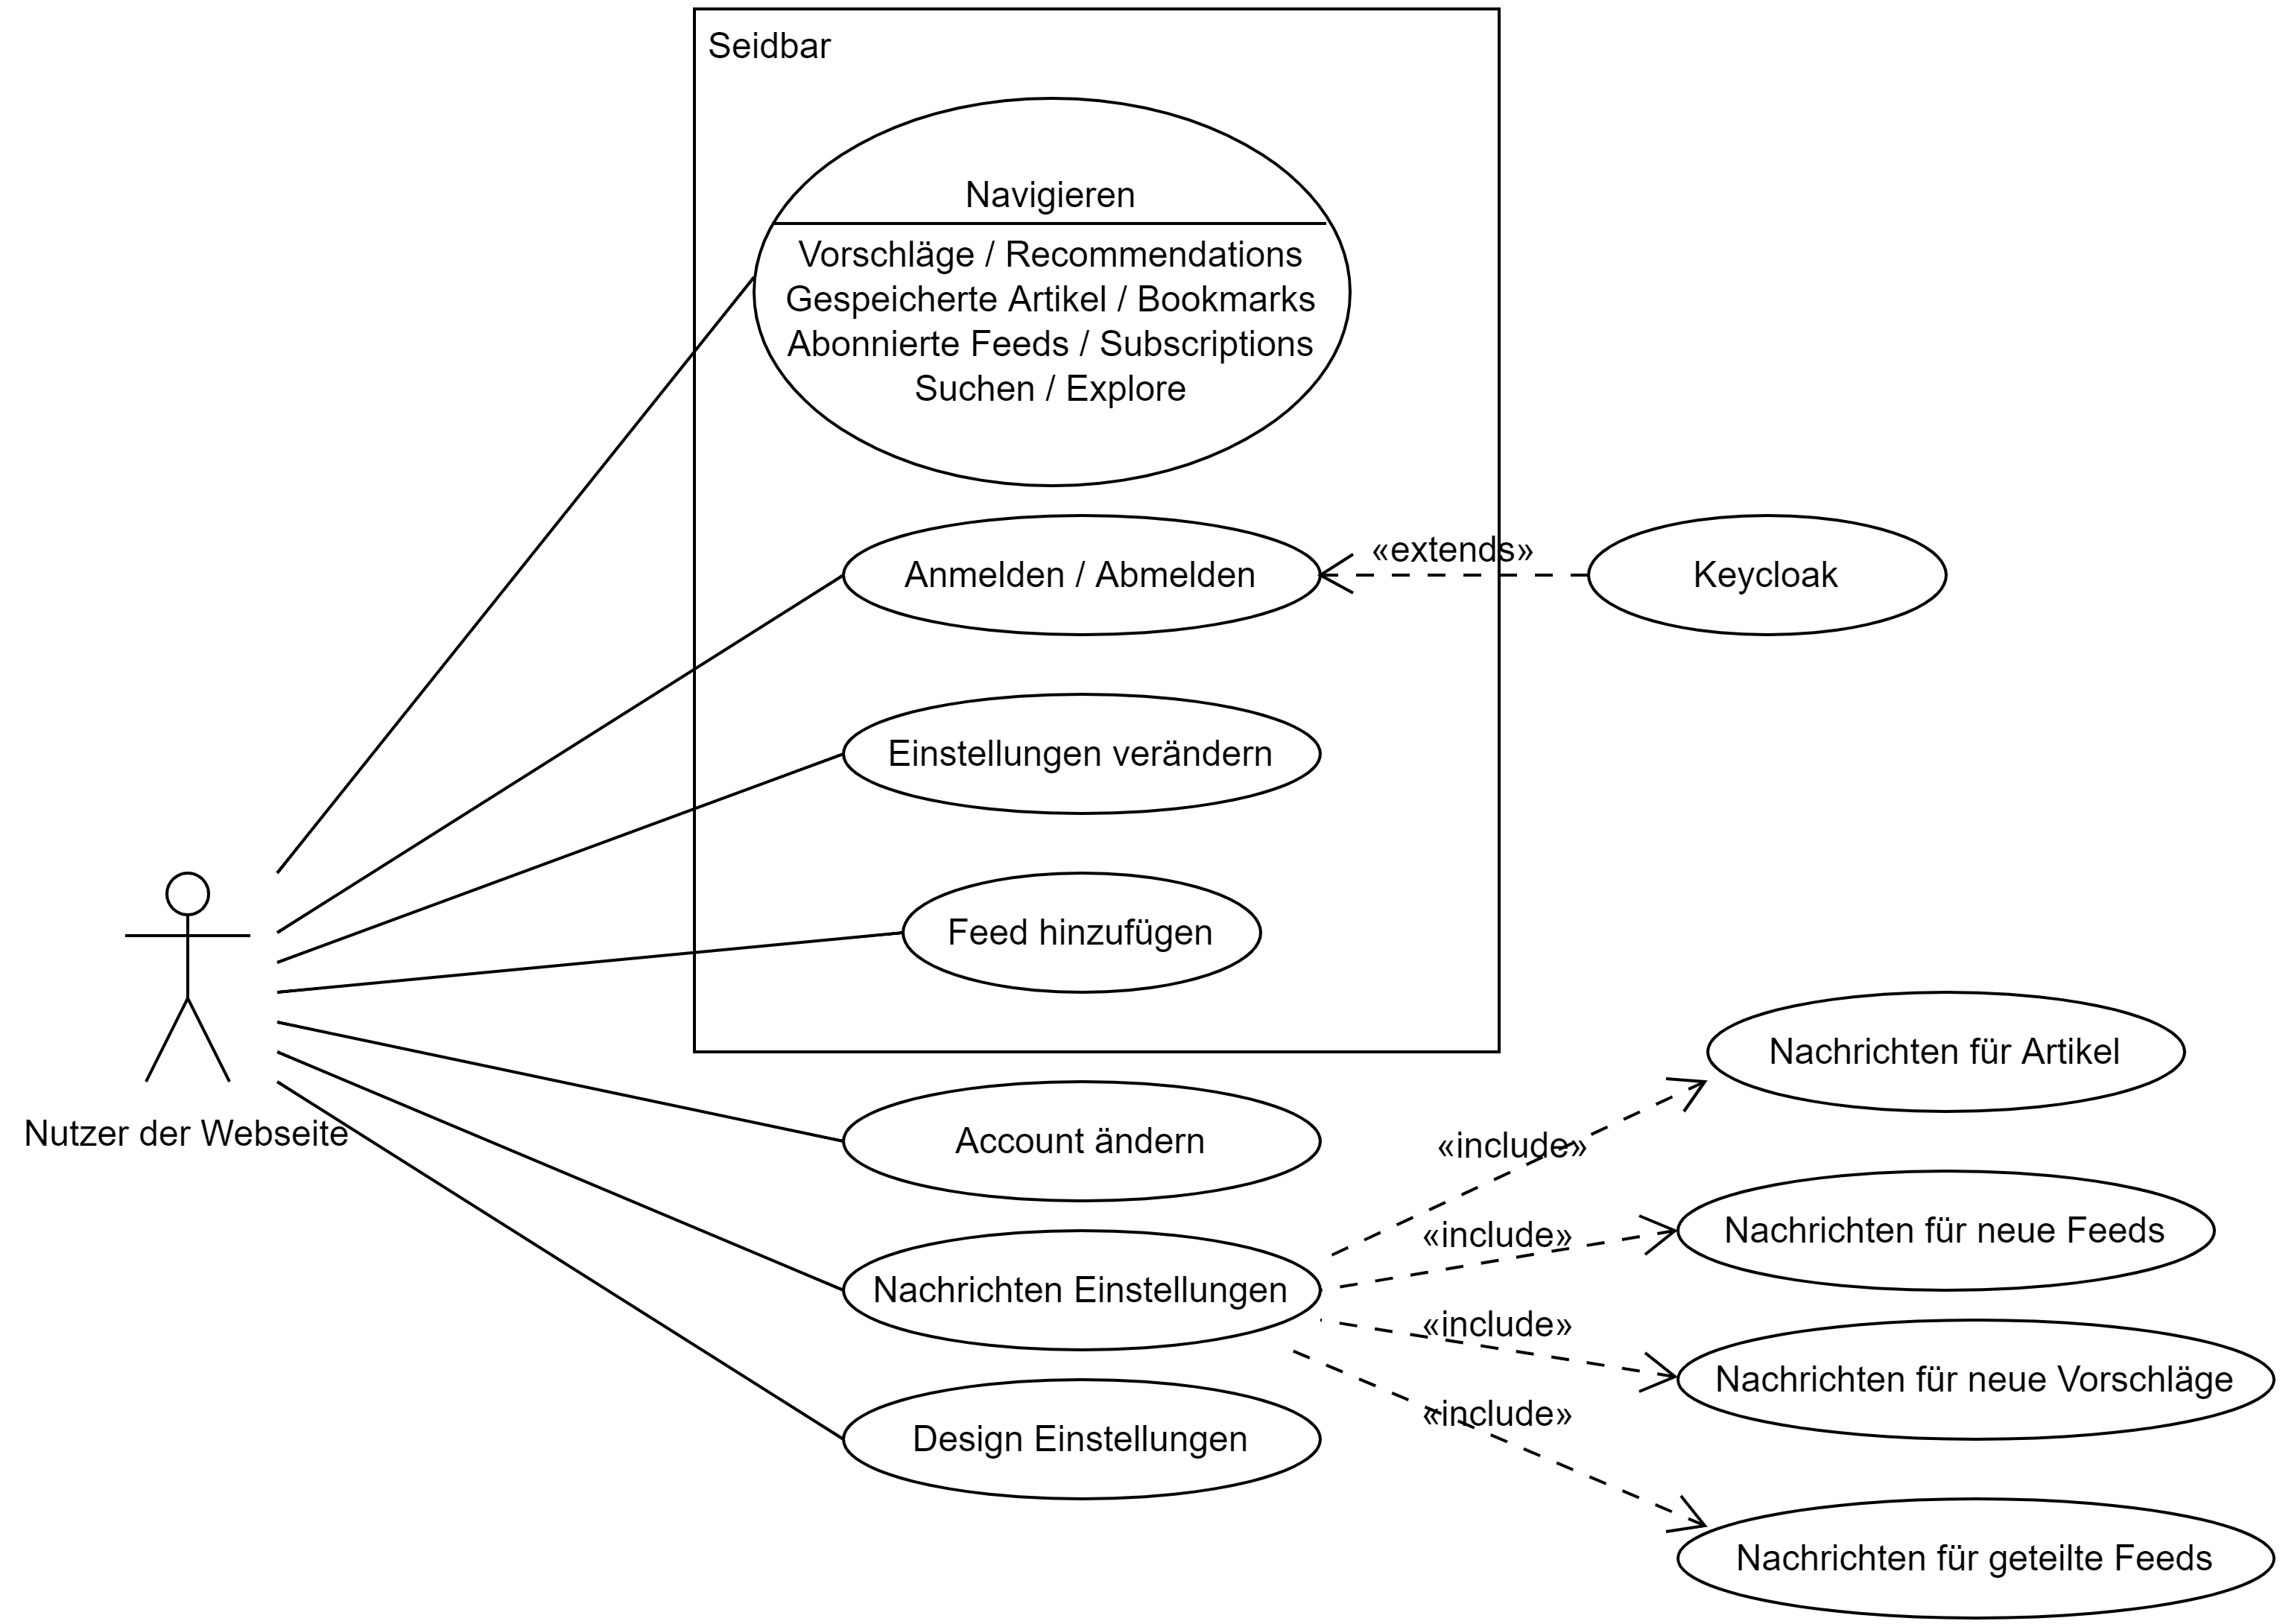
\includegraphics[width=\linewidth]{umlUsecaseSettings.png}
    \caption{Usecase Diagramm der Einstellungsseite}
    \label{fig:usecaseSettings}
\end{figure}


Es wurde ebenfalls ein Usecase Diagramm der Artikelseite angelegt. Auf diese Seite
wird der Nutzer weitergeleitet, falls er aus der Übersichtsseite einen Artikel anschaut.
Der Usecase der Artikelseite ist in der Abbilung~\ref{fig:usecaseView} dargestellt.
\begin{figure}
    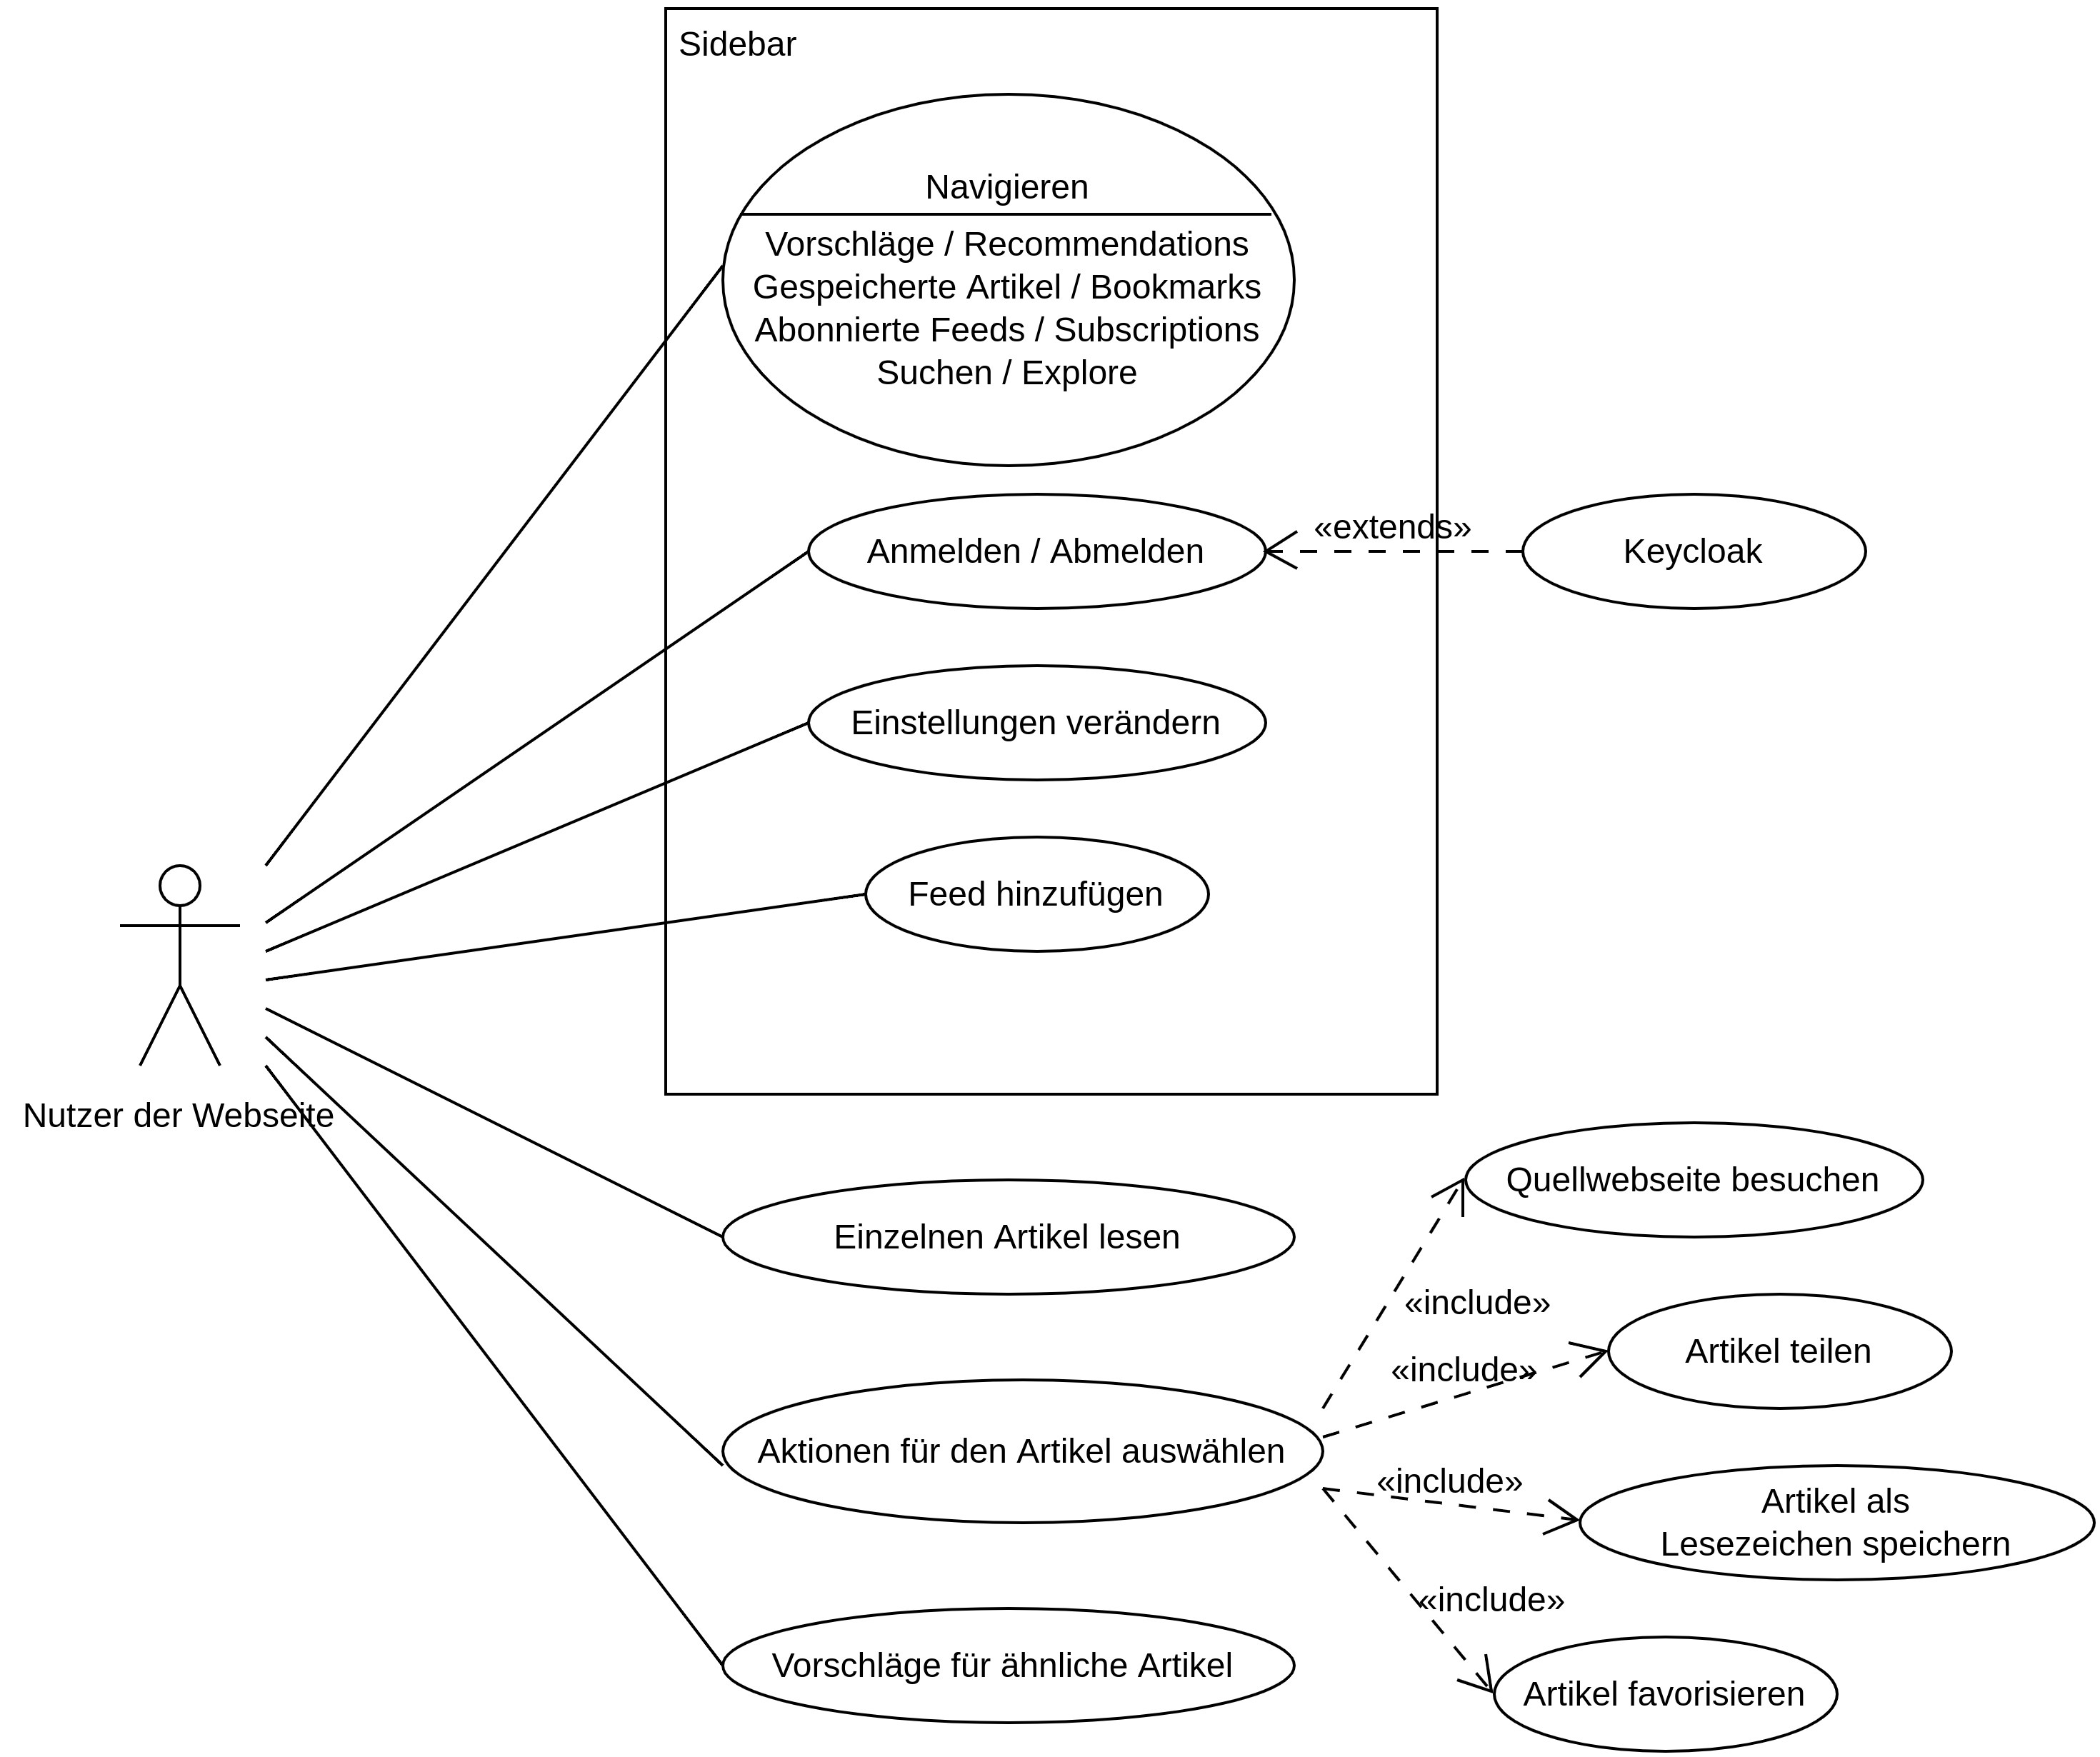
\includegraphics[width=\linewidth]{umlUsecaseView.png}
    \caption{Usecase Diagramm der Artikelseite}
    \label{fig:usecaseView}
\end{figure}
Zudem kann ein Benutzer verschiedene Aktionen auswählen, dazu zählen Quellwebseite des Artikels besuchen, Artikel teilen, Artikel als 
Lesezeichen speichern und Artikel favorisieren. Unterhalb der Aktionen werden Artikel angezeigt, die aufgrund bisheriger Präferenzen und 
favorisierten Artikeln passen könnten.
